\documentclass[11pt,a4paper]{article}

% ---------------------------------------------------------------------------
% Child-selection determinants and unstable cores in sequential distributive
% futile cycles.
%
% Author metadata: set the three macros below before submission.
% They are deliberately left blank in this version.
% ---------------------------------------------------------------------------
\newcommand{\PaperAuthor}{}
\newcommand{\PaperAffiliation}{}
\newcommand{\PaperDate}{14 September 2026}

\usepackage[T1]{fontenc}
\usepackage[utf8]{inputenc}
\usepackage{lmodern}
\usepackage{microtype}
\usepackage[a4paper,margin=1.05in]{geometry}
\usepackage{amsmath,amssymb,amsthm,mathtools}
\usepackage{booktabs}
\usepackage{array}
\usepackage{enumitem}
\usepackage{xcolor}
\usepackage{graphicx}
\usepackage[obeyspaces,spaces]{url}
\usepackage[numbers,sort&compress]{natbib}
\usepackage[colorlinks=true,linkcolor=blue!55!black,citecolor=blue!55!black,urlcolor=blue!55!black]{hyperref}
\hypersetup{pdftitle={Child-selection determinants and unstable cores in sequential distributive futile cycles},
  pdfkeywords={multisite phosphorylation, futile cycle, child selection, unstable core, D-stability, Routh--Hurwitz, formal verification, Lean}}

\DeclareUrlCommand\lean{\urlstyle{tt}}
\setlist{itemsep=2pt,topsep=3pt}
\setlength{\emergencystretch}{1.5em}
\graphicspath{{figures/}}

\theoremstyle{plain}
\newtheorem{theorem}{Theorem}[section]
\newtheorem{proposition}[theorem]{Proposition}
\newtheorem{lemma}[theorem]{Lemma}
\newtheorem{corollary}[theorem]{Corollary}
\theoremstyle{definition}
\newtheorem{definition}[theorem]{Definition}
\newtheorem{example}[theorem]{Example}
\newtheorem{question}[theorem]{Question}
\theoremstyle{remark}
\newtheorem{remark}[theorem]{Remark}

\newcommand{\R}{\mathbb R}
\newcommand{\C}{\mathbb C}
\newcommand{\Z}{\mathbb Z}
\newcommand{\N}{\mathbb N}
\newcommand{\cS}{\mathcal S}
\newcommand{\cE}{\mathcal E}
\newcommand{\cC}{\mathcal C}
\newcommand{\cG}{\mathcal G}
\newcommand{\Aminus}{A_{-}}
\newcommand{\own}{\jmath}
\newcommand{\T}{\mathsf T}
\DeclareMathOperator{\diag}{diag}
\DeclareMathOperator{\Ree}{Re}
\DeclareMathOperator{\Imm}{Im}
\DeclareMathOperator{\spec}{spec}
\DeclareMathOperator{\im}{im}
\DeclareMathOperator{\rank}{rank}
\DeclareMathOperator{\sgn}{sgn}

\title{Child-selection determinants and unstable cores\\in sequential distributive futile cycles}
\author{\PaperAuthor\\[2pt]\small\PaperAffiliation}
\date{\PaperDate}

\begin{document}
\maketitle

\begin{abstract}
Vassena and Stadler localized instability in reaction networks to \emph{unstable cores}: minimal child-selection matrices with an eigenvalue of positive real part. For the sequential distributive dual futile cycle they found exactly three unstable cores, all \emph{unstable-positive}, all with determinant of modulus one, and conjectured that the same picture persists for the $n$-site cycle built by adding phosphorylation steps. We settle this conjecture by separating its two assertions. The determinant assertion holds in a class much larger than the futile cycles: every child-selection matrix of an elementary enzyme-conversion system, singular or not, has determinant $0$ or $\pm1$. The structural assertion fails in two ways. For every $n\ge3$ the cycle contains a fixed six-species minimal \emph{unstable-negative} core, and for every $n\ge2$ it contains a minimal unstable-positive core of dimension $2n+1$ that specializes at $n=2$ to one of the three dual-cycle cores and remains minimally unstable under every positive column scaling; the literal dimensions of minimal positive cores are therefore unbounded. A five-species restriction of the negative witness is strictly stable at unit scaling yet is a $D$-unstable-negative core, so ordinary and scaling-invariant minimality differ within one network. For the positive family we derive a scalar return equation that identifies the spectral abscissa for arbitrary rates and losses, giving exact rate comparisons and a sharp loss threshold; at unit rates the unstable eigenvalue is $W(n-1)/(2(n-1))+O(W(n-1)^2/(n-1)^2)\sim\log n/(2n)$, so the instability weakens as the cores grow. An explicit saturating-kinetic model of the complete three-step network realizes an unstable positive equilibrium with exactly three eigenvalues in the open right half-plane. The determinant theorem, both core families and the scaling statements are verified in Lean~4; the rate-dependence, asymptotic and kinetic results have conventional proofs with exact rational certificates that a supplied script replays.
\end{abstract}

\section{Introduction}\label{sec:intro}

Multisite phosphorylation cycles are among the most studied motifs of cell signalling. A substrate carrying $n$ modification sites is phosphorylated by a kinase and dephosphorylated by a phosphatase, sequentially and distributively, through enzyme--substrate intermediates \citep{Markevich2004,Gunawardena2005,ConradiShiu2018}. The $n$-site cycle exhibits bistability for $n=2$ \citep{Markevich2004,HellRendall2015}, has at most $2n-1$ positive steady states, and the number of steady states it can support grows without bound with $n$ \citep{WangSontag2008,ThomsonGunawardena2009,FeliuRendallWiuf2020}; the processive variant is globally stable \citep{Rao2017}, and mixed mechanisms oscillate \citep{SuwanmajoKrishnan2015,ConradiMinchevaShiu2019}. Whether the sequential distributive dual cycle can oscillate under mass action was a long-standing open question \citep{Errami2015,ConradiShiu2018}; it was recently shown that it cannot, whereas parameter-rich kinetics on the same network do admit a Hopf bifurcation \citep{Vassena2026}.

A structural approach to such questions decides dynamical properties from the network alone, independently of rate constants \citep{Clarke1980,MinchevaRoussel2007,Feinberg2019}. The notion we use is the \emph{child selection} of Brehm and Fiedler \citep{BrehmFiedler2018,Vassena2020}: a set of species, each assigned a distinct reaction in which it is a reactant; the corresponding columns of the stoichiometric matrix form a square \emph{child-selection matrix}. Vassena and Stadler \citep{VassenaStadler2024} proved that if some child-selection matrix becomes Hurwitz-unstable after multiplication by a positive diagonal matrix, then every parameter-rich kinetics on the network admits an unstable positive equilibrium, and they called a minimal such matrix an \emph{unstable core}. Cores come in two signs. In dimension $k$ an unstable core with $\sgn\det=(-1)^{k-1}$ is \emph{unstable-positive} and one with $\sgn\det=(-1)^k$ is \emph{unstable-negative}; the sign distinguishes positive feedback, which typically produces a real unstable eigenvalue, from negative feedback, which produces an unstable complex pair.

In Supplementary Example D of \citep{VassenaStadler2024} the framework is applied to the dual futile cycle. An exhaustive search over its child selections finds exactly three unstable cores, which the authors call $S_1$, $S_2$ and $S_3$: two of dimension five, related by the kinase--phosphatase symmetry, and one of dimension six. All three are unstable-positive, and every invertible child-selection matrix of the network has determinant $\pm1$. The example closes with a conjecture for the $n$-site cycle, ``built iteratively by adding further distributive and sequential phosphorylation steps'': that only unstable-positive feedbacks with matrices as $S_1=S_2$ or $S_3$ appear, and that $|\det S[\kappa]|=1$ for all invertible child-selection matrices.

\paragraph{Results.}
We resolve this conjecture. Its two assertions have different fates.

\begin{enumerate}[label=(\alph*)]
\item \emph{Determinants.} Every child-selection matrix of the $n$-site cycle has determinant $0$, $1$ or $-1$, for every $n$ and including singular and empty selections (Theorem~\ref{thm:det}). The proof uses only that each enzyme--substrate intermediate has one binding reaction and returns its enzyme, so the theorem holds for all elementary enzyme-conversion systems in the sense of Section~\ref{sec:setting}: cascades, several enzymes per substrate and mixed mechanisms included.
\item \emph{A negative core.} For every $n\ge3$ the cycle contains a six-species child $\Aminus$, independent of $n$, that is a minimal unstable-negative core with $\det\Aminus=1$ (Theorem~\ref{thm:negative}). The all-positive assertion therefore fails from three sites onward. Its unstable eigenvalues form a complex pair.
\item \emph{Unbounded positive cores.} For every $n\ge2$ the cycle contains a minimal unstable-positive core $A_n$ of dimension $2n+1$ with $\det A_n=1$ (Theorem~\ref{thm:positive}). At $n=2$, $A_2$ is exactly the core $S_2$ of Example D, so $(A_n)$ is the natural extension of that motif; but its dimension grows without bound, so no finite list of matrices describes the positive cores of all cycles. Every $A_nD$ with $D$ positive diagonal is again a minimal unstable-positive core.
\item \emph{Two notions of minimality.} The five-species restriction $B$ of $\Aminus$ is strictly Hurwitz stable, yet $BD_*$ is unstable for $D_*=\diag(1,1,2,1,2)$ and every proper restriction of $B$ is nonunstable under every positive scaling (Theorem~\ref{thm:five}). So $B$ is a $D$-unstable-negative core in the sense of \citep{VassenaStadler2024} while $\Aminus$ is an unstable core that is not $D$-minimal. Ordinary and scaling-invariant minimality differ within the same network.
\item \emph{Rate dependence.} For the positive family with arbitrary column rates $d_i>0$ and independent losses $\eta_i\ge0$, the spectral abscissa is the unique root of an explicit scalar return equation (Theorem~\ref{thm:return}). It increases strictly in every rate, is homogeneous of degree one, and independent losses stabilize exactly when a product of gain fractions drops below one. At unit rates the unstable eigenvalue satisfies $\alpha_n=W(n-1)/(2(n-1))+O(W(n-1)^2/(n-1)^2)\sim\log n/(2n)$, with finite two-sided Lambert-function brackets (Proposition~\ref{prop:asymptotic}); the cores grow while their instability margin vanishes. For $n=10$ the core has three eigenvalues in the open right half-plane although its positive real eigenvalue is unique.
\item \emph{A full-network realization.} A complete kinetic model of the three-step cycle, with all twelve species, all eighteen reactions, balanced positive flux and explicit saturating rate laws, has an unstable positive equilibrium whose Jacobian has exactly three eigenvalues of positive real part and three conservation zeros (Proposition~\ref{prop:kinetic}).
\end{enumerate}

\paragraph{What is not claimed.}
The negative core and the positive family refute the conjecture as stated, with ``matrices as $S_1=S_2$ or $S_3$'' read literally. They do not settle a classification of positive cores up to subdivision of the long cycle, which is a different and interesting question (Section~\ref{sec:discussion}). Minimality throughout is with respect to proper principal restrictions, as in \citep{VassenaStadler2024}, not smallest dimension among all children. A child-selection matrix is not the Jacobian of any particular kinetics; the kinetic example of Section~\ref{sec:kinetics} is included precisely to separate the two. No mass-action Hopf bifurcation or periodic orbit is asserted for the $n$-site cycle; for the dual cycle under mass action, none exists \citep{Vassena2026}.

\paragraph{Method.}
The determinant theorem is a two-step reduction: a unit-determinant block operation eliminates the selected intermediates, and a sign change on the enzyme rows turns every remaining column into a signed-incidence column with at most one $+1$ and one $-1$, whose determinants are $0$ or $\pm1$ by cofactor induction. Instability of the negative core follows from a reciprocal-root identity for its characteristic quintic and an explicit polynomial eigenvector; minimality follows from the cycle structure of the matrix together with one exact Lyapunov certificate. The positive family is conjugate by a diagonal sign matrix to an irreducible Metzler matrix consisting of a long cycle and a two-cycle sharing one hub; instability comes from an intermediate-value root, minimality under all scalings from a norm-contraction argument along the cycle, and the return equation from propagating an eigenvector around both cycles. The five-species $D$-core uses a logarithmic-derivative certificate on the imaginary axis. All exact numbers in the paper are replayed by the supplied script \path{check_paper.py}.

\paragraph{Verification.}
The determinant theorem, the negative and positive core families with their all-$n$ source embeddings, the refutations, the all-scaling minimality of $A_nD$, and the five-species $D$-core are verified in Lean~4 with Mathlib \citep{Lean4,Mathlib}; Appendix~\ref{app:formal} lists the declarations. The return equation and its corollaries, the Lambert asymptotics, the exact unstable-root counts and the kinetic realization are conventional proofs supported by exact rational certificates.

\paragraph{Organization.}
Section~\ref{sec:setting} fixes the class of networks, child selections, cores and the $n$-site cycle, and restates the conjecture. Section~\ref{sec:results} collects the theorems. Sections~\ref{sec:det}--\ref{sec:positive} prove the determinant theorem, the negative cores and the positive family. Section~\ref{sec:rates} treats rates, losses and asymptotics, Section~\ref{sec:kinetics} the kinetic realization. Section~\ref{sec:discussion} discusses the consequences and open questions. Appendix~\ref{app:formal} is the formal source map and Appendix~\ref{app:cert} lists the exact certificates.

\section{Setting}\label{sec:setting}

\subsection{Elementary enzyme-conversion systems}
Let $\cS$, $\cE$ and $\cC$ be disjoint finite sets of \emph{substrates}, \emph{enzymes} and \emph{intermediates}. Each intermediate $c\in\cC$ has an input substrate $s(c)\in\cS$, an output substrate $t(c)\in\cS$ and an enzyme $e(c)\in\cE$, and carries three reactions
\begin{equation}\label{eq:arms}
s(c)+e(c)\xrightarrow{\;b_c\;}c,\qquad
c\xrightarrow{\;u_c\;}s(c)+e(c),\qquad
c\xrightarrow{\;v_c\;}t(c)+e(c),
\end{equation}
binding, unbinding and conversion. All stoichiometric coefficients are one, every intermediate belongs to exactly one such arm, and the arm returns its own enzyme. Nothing else is assumed: several intermediates may share an input, an enzyme may serve many arms, $s(c)=t(c)$ is allowed, and the arms may form chains, cycles or cascades. We call such a network an \emph{elementary enzyme-conversion system}. Its reactant matrix $Y$, product matrix $\widetilde Y$ and stoichiometric matrix $S=\widetilde Y-Y$ have rows indexed by species $\cS\sqcup\cE\sqcup\cC$ and columns by the $3|\cC|$ reactions.

\subsection{Child selections and cores}
\begin{definition}[Child selection]\label{def:child}
A \emph{child selection} consists of a finite index set $I$, distinct species $m_i$ ($i\in I$) and distinct reactions $\own(i)$ with $Y_{m_i,\own(i)}>0$, that is, $m_i$ is a reactant of $\own(i)$. Its \emph{child-selection matrix} is
\begin{equation}\label{eq:child}
A_{ij}=S_{m_i,\own(j)},\qquad i,j\in I .
\end{equation}
Species $m_j$ is the \emph{owner} of column $j$. A \emph{restriction} of $A$ to $I'\subseteq I$ keeps the owners in $I'$ together with their columns; it is the principal submatrix $A[I']$ and is itself a child-selection matrix.
\end{definition}

This is the child selection of \citep{BrehmFiedler2018,VassenaStadler2024}, with the empty selection included and no invertibility required. Tying each column to its owner is what makes restrictions principal.

Throughout, a real square matrix is \emph{unstable} if it has an eigenvalue with strictly positive real part, and \emph{nonunstable} otherwise; nonunstable matrices may have eigenvalues on the imaginary axis, including zero, so nonunstability is weaker than Hurwitz stability. A \emph{positive scaling} of $A$ is $AD$ with $D$ a positive diagonal matrix; it multiplies each column by a positive rate. $A$ is \emph{$D$-unstable} if $AD$ is unstable for some positive $D$, and \emph{$D$-nonunstable} if $AD$ is nonunstable for every positive $D$ \citep{Cross1978,Kushel2019}.

\begin{definition}[Cores]\label{def:core}
A child-selection matrix $A$ is an \emph{unstable core} if $A$ is unstable and every proper restriction of $A$ is nonunstable. It is a \emph{$D$-unstable core} if $A$ is $D$-unstable and every proper restriction is $D$-nonunstable. In dimension $k$ a nonsingular core is \emph{positive} if $\sgn\det A=(-1)^{k-1}$ and \emph{negative} if $\sgn\det A=(-1)^{k}$. Positive scaling preserves the sign of the determinant, so the same convention applies to $D$-unstable cores.
\end{definition}

The sign convention is that of \citep{VassenaStadler2024}: a positive core has the determinant sign of $-\!I$ with one sign reversed, as produced by a single positive feedback loop. Minimality is principal: a core may properly contain a smaller unstable child whose owners are not a subset of its own.

\subsection{The \texorpdfstring{$n$}{n}-site futile cycle}
Fix $n\ge1$. The $n$-site sequential distributive futile cycle has substrates $S_0,\dots,S_n$ (the substrate with $i$ phosphate groups), a kinase $K$, a phosphatase $F$, and intermediates $C_0,\dots,C_{n-1}$ and $D_1,\dots,D_n$, with arms
\begin{align}\label{eq:network}
S_i+K\ \xrightleftharpoons[K_i^u]{K_i^b}\ C_i\ \xrightarrow{K_i^v}\ S_{i+1}+K \qquad&(0\le i<n),\\
S_i+F\ \xrightleftharpoons[F_i^u]{F_i^b}\ D_i\ \xrightarrow{F_i^v}\ S_{i-1}+F \qquad&(1\le i\le n).\nonumber
\end{align}
It has $3n+3$ species and $6n$ reactions and is an elementary enzyme-conversion system with $s(C_i)=S_i$, $t(C_i)=S_{i+1}$, $e(C_i)=K$, $s(D_i)=S_i$, $t(D_i)=S_{i-1}$, $e(D_i)=F$. The dual cycle of \citep{VassenaStadler2024} is $n=2$ with $(A,B,C,E_1,E_2,I_1,I_2,I_3,I_4)=(S_0,S_1,S_2,K,F,C_0,D_1,C_1,D_2)$ and reactions $1,\dots,12$ equal to $K_0^b,K_0^u,K_0^v,F_1^b,F_1^u,F_1^v,K_1^b,K_1^u,K_1^v,F_2^b,F_2^u,F_2^v$. The symbolic reaction names avoid any dependence on reaction numbering. Figure~\ref{fig:source} shows $n=3$.

\begin{figure}[htbp]
\centering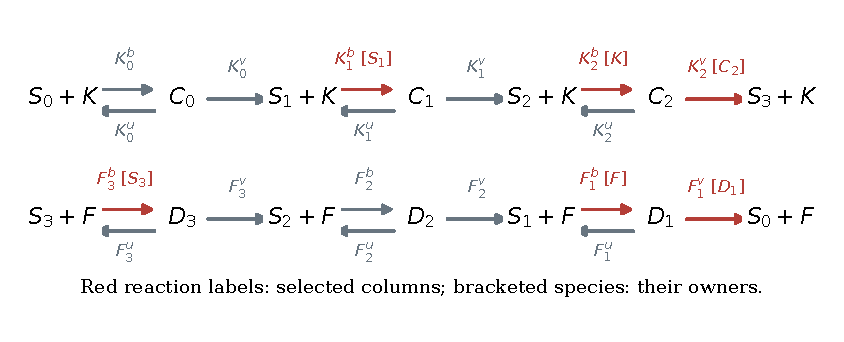
\includegraphics[width=\linewidth]{source_network.pdf}
\caption{The three-site cycle with all eighteen reactions. Repeated substrate and enzyme names denote the same species. The six red reactions and their bracketed owners define the negative core $\Aminus$ of Section~\ref{sec:negative}; all other reactions remain part of the network.}
\label{fig:source}
\end{figure}

\subsection{The conjecture of Example D}\label{sec:conjecture}
In the notation above, the three unstable cores of the dual cycle found in \citep{VassenaStadler2024} are the children
\begin{equation}\label{eq:VScores}
\begin{aligned}
S_1&: (S_0,K,C_1,S_1,D_1)\ \text{owning}\ (K_0^b,K_1^b,K_1^v,F_1^b,F_1^v),\\
S_2&: (S_2,F,D_1,S_1,C_1)\ \text{owning}\ (F_2^b,F_1^b,F_1^v,K_1^b,K_1^v),\\
S_3&: (S_0,K,C_1,S_2,F,D_1)\ \text{owning}\ (K_0^b,K_1^b,K_1^v,F_2^b,F_1^b,F_1^v),
\end{aligned}
\end{equation}
with matrices
\[
S_1=S_2=\begin{pmatrix}-1&0&0&0&1\\-1&-1&1&0&0\\0&1&-1&0&0\\0&-1&0&-1&0\\0&0&0&1&-1\end{pmatrix},\qquad
S_3=\begin{pmatrix}-1&0&0&0&0&1\\-1&-1&1&0&0&0\\0&1&-1&0&0&0\\0&0&1&-1&0&0\\0&0&0&-1&-1&1\\0&0&0&0&1&-1\end{pmatrix}.
\]
(The script \path{check_paper.py} rebuilds these from \eqref{eq:network} and compares them with the displayed matrices.) $S_1$ and $S_2$ are exchanged by the symmetry $S_i\leftrightarrow S_{n-i}$, $K\leftrightarrow F$, $C_i\leftrightarrow D_{n-i}$. The conjecture asserts that for every $n$: (C1) only unstable-positive cores appear, with matrices as $S_1=S_2$ or $S_3$; and (C2) every invertible child-selection matrix has determinant $\pm1$. We prove (C2) in a strengthened form and refute (C1) in two independent ways.

\section{Main results}\label{sec:results}

\begin{theorem}[Unit determinants]\label{thm:det}
Every child-selection matrix of an elementary enzyme-conversion system, including singular and empty selections, has determinant $0$, $1$ or $-1$. In particular this holds for the $n$-site futile cycle for every $n\ge1$.
\end{theorem}

\begin{theorem}[A negative core in every cycle with at least three sites]\label{thm:negative}
For every $n\ge3$, the child of the $n$-site cycle with owners and reactions
\begin{equation}\label{eq:negowners}
\begin{array}{c|cccccc}
\text{species}&S_1&S_3&K&F&C_2&D_1\\
\text{owned reaction}&K_1^b&F_3^b&K_2^b&F_1^b&K_2^v&F_1^v
\end{array}
\end{equation}
has the matrix $\Aminus$ of \eqref{eq:Aminus} below, independent of $n$. $\Aminus$ is an unstable core with $\det\Aminus=1=(-1)^6$, hence unstable-negative. Its unstable eigenvalues form a nonreal conjugate pair.
\end{theorem}

\begin{theorem}[Unbounded positive cores]\label{thm:positive}
For every $n\ge2$, the child of the $n$-site cycle with ordered owners
\begin{equation}\label{eq:posorder}
(F,\ S_1,C_1,\ S_2,C_2,\ \dots,\ S_{n-1},C_{n-1},\ S_n,\ D_1)
\end{equation}
owning $F_1^b$, $K_i^b$ and $K_i^v$ for $1\le i<n$, $F_n^b$ and $F_1^v$ respectively, has dimension $2n+1$, matrix $A_n$ with $\det A_n=1=(-1)^{2n}$, and is an unstable-positive core. Moreover, for every positive diagonal $D$, $A_nD$ has a positive real eigenvalue and every proper restriction of $A_nD$ is nonunstable, so $A_nD$ is again an unstable-positive core and $A_n$ is a $D$-unstable core. At $n=2$, $A_2$ is the core $S_2$ of \eqref{eq:VScores}.
\end{theorem}

\begin{theorem}[A five-species $D$-unstable-negative core]\label{thm:five}
For every $n\ge3$, the restriction $B=\Aminus[S_1,S_3,K,F,C_2]$ of the child \eqref{eq:negowners} is strictly Hurwitz stable, while $BD_*$ with $D_*=\diag(1,1,2,1,2)$ has exactly two eigenvalues in the open right half-plane, a nonreal conjugate pair, and every proper restriction of $B$ is $D$-nonunstable. Thus $B$ is a $D$-unstable core with $\det B=-1=(-1)^5$, a $D$-unstable-negative core, and $\Aminus$ is an unstable core that is not a $D$-unstable core.
\end{theorem}

\begin{corollary}[Resolution of the conjecture]\label{cor:resolution}
Assertion \textup{(C2)} holds for all $n$, and in the stronger form of Theorem~\ref{thm:det}. Assertion \textup{(C1)} fails: for $n\ge3$ an unstable-negative core exists, and for every bound $M$ there is an $n$ whose cycle contains a minimal unstable-positive core of dimension exceeding $M$.
\end{corollary}

The remaining results concern the positive family quantitatively and the full network kinetically; they are stated in Sections~\ref{sec:rates} and~\ref{sec:kinetics}: the return equation (Theorem~\ref{thm:return}) with its rate and loss corollaries, the asymptotics of the unit-rate eigenvalue (Proposition~\ref{prop:asymptotic}), and the kinetic realization (Proposition~\ref{prop:kinetic}).

\begin{remark}[Evidence levels]
Theorems~\ref{thm:det}--\ref{thm:five} and Corollary~\ref{cor:resolution} are verified in Lean~4 as stated, with the source network \eqref{eq:network} and the children \eqref{eq:negowners}, \eqref{eq:posorder} defined literally; the only exception is the exact count of two unstable roots in Theorems~\ref{thm:negative} and~\ref{thm:five}, which is an exact Routh computation (Appendix~\ref{app:cert}) whose existence part is formalized. Theorem~\ref{thm:return}, Proposition~\ref{prop:asymptotic} and Proposition~\ref{prop:kinetic} are conventional proofs. Appendix~\ref{app:formal} gives the precise map.
\end{remark}

\section{The determinant theorem}\label{sec:det}

\begin{lemma}[Signed-incidence determinants]\label{lem:incidence}
Let $H$ be a square integer matrix with entries in $\{0,1,-1\}$ such that every column contains at most one entry $+1$ and at most one entry $-1$. Then $\det H\in\{0,1,-1\}$.
\end{lemma}
\begin{proof}
Induct on the order, the empty determinant being one. If some column has at most one nonzero entry, expand along it: the determinant is $0$ or $\pm$ a minor, and the minor satisfies the same hypotheses. Otherwise every column contains exactly one $+1$ and one $-1$, so every column sum is zero, the all-ones row vector is a left null vector, and $\det H=0$.
\end{proof}

The lemma is the classical total unimodularity of directed-graph incidence matrices \citep[Chapter~19]{Schrijver1986}, in the only form needed here: a column with one entry of each sign is an arc, a column with a single entry is an arc with one end outside the selected vertex set.

\begin{lemma}[Intermediate elimination]\label{lem:elimination}
Let $A=\begin{pmatrix}B&W\\C&-I_q\end{pmatrix}$ with square $B$. Then $\det A=(-1)^q\det(B+WC)$.
\end{lemma}
\begin{proof}
$A\begin{pmatrix}I&0\\C&I\end{pmatrix}=\begin{pmatrix}B+WC&W\\0&-I_q\end{pmatrix}$, and the multiplier has determinant one.
\end{proof}

\begin{proof}[Proof of Theorem~\ref{thm:det}]
Let $A$ be the matrix of a child selection with index set $I$. Split $I=U\sqcup V$, where $U$ indexes the selected substrates and enzymes (\emph{free} species) and $V$ the selected intermediates, and order $U$ first, permuting rows and their owned columns together, which does not change the determinant. A free species is a reactant only of binding reactions, so each $j\in U$ owns a binding column $b_{c_j}$. An intermediate $c$ is a reactant only of $u_c$ and $v_c$, so each $k\in V$ owns an outgoing column of its own intermediate $c_k$; write $o_k\in\{u_{c_k},v_{c_k}\}$. Since reactions are distinct, $k\mapsto c_k$ is injective on $V$.

In this order $A=\begin{pmatrix}B&W\\C&-I_q\end{pmatrix}$ with $q=|V|$: the block $-I_q$ records that $o_k$ consumes exactly one $c_k$ and no other selected intermediate; $C_{kj}=1$ if $c_k=c_j$ and $0$ otherwise, because $b_{c_j}$ produces $c_j$ only; $B_{ij}=S_{m_i,b_{c_j}}$ and $W_{ik}=S_{m_i,o_k}$ for free $m_i$. By Lemma~\ref{lem:elimination}, $\det A=(-1)^q\det(B+WC)$.

Consider column $j\in U$ of $B+WC$. If $c_j$ is not a selected intermediate, the column of $C$ is zero and the reduced column is the binding column $-e_{s(c_j)}-e_{e(c_j)}$ restricted to the free rows. If $c_j=c_k$ for a (unique) $k\in V$, the reduced column is the sum of the binding column and the column of $o_k$ restricted to free rows:
\begin{equation}\label{eq:reduced}
(-e_{s}-e_{e})+(e_{s}+e_{e})=0\quad\text{if }o_k=u_{c_j},\qquad
(-e_{s}-e_{e})+(e_{t}+e_{e})=e_{t}-e_{s}\quad\text{if }o_k=v_{c_j},
\end{equation}
with $s=s(c_j)$, $t=t(c_j)$, $e=e(c_j)$, and where $e_x$ is read as zero when $x$ is not selected. Now multiply every enzyme row by $-1$. The unmatched binding column becomes $e_{e}-e_{s}$, and the two cases in \eqref{eq:reduced} are unchanged. Every column of the resulting matrix $H$ is therefore $0$, or a difference $e_a-e_b$ of two coordinate vectors, possibly with $a=b$ or with one or both coordinates absent. Hence $H$ satisfies the hypothesis of Lemma~\ref{lem:incidence}, $\det H\in\{0,\pm1\}$, and $\det(B+WC)=\pm\det H$. Combined with the factor $(-1)^q$ this proves $\det A\in\{0,1,-1\}$.
\end{proof}

\begin{remark}
The proof uses only unit stoichiometry, a single binding reaction per intermediate and the return of the enzyme. It applies unchanged to networks in which one substrate is bound by several enzymes, to several substrates sharing an enzyme, and to processive or mixed mechanisms as long as each intermediate is formed by one binding step. Cascades in which a modified substrate acts as the enzyme of the next layer violate the disjointness of roles and are not covered as stated. The structural reason is that at zero frequency an intermediate transmits its binding column unchanged to its outgoing reaction, so the selected intermediates collapse to incidence relations among free species. The determinant is a zero-frequency invariant only: the same reduction with $z\neq0$ carries a factor $1/(z+1)$ per eliminated intermediate and is not spectrum preserving, which is why unit determinants coexist with the complex-pair instability of Section~\ref{sec:negative}.
\end{remark}

\section{Negative cores}\label{sec:negative}

\subsection{The six-species witness}
For $n\ge3$ the six reactions in \eqref{eq:negowners} are distinct and each owner is a reactant of its reaction. Reading off the columns $K_1^b,F_3^b,K_2^b,F_1^b,K_2^v,F_1^v$ at the rows $S_1,S_3,K,F,C_2,D_1$ gives
\begin{equation}\label{eq:Aminus}
\Aminus=\begin{pmatrix}
-1&0&0&-1&0&0\\
0&-1&0&0&1&0\\
-1&0&-1&0&1&0\\
0&-1&0&-1&0&1\\
0&0&1&0&-1&0\\
0&0&0&1&0&-1
\end{pmatrix},\qquad \det\Aminus=1 .
\end{equation}
No entry involves $n$: the species and reactions used exist for every $n\ge3$ and no other reaction is selected, so $\Aminus$ is the same matrix in every such cycle. (At $n=2$ the reaction $F_3^b$ does not exist; this is consistent with the exhaustive search of \citep{VassenaStadler2024}, which found no negative core in the dual cycle.)

Direct expansion gives
\begin{equation}\label{eq:pminus}
\det(zI-\Aminus)=z^6+6z^5+13z^4+12z^3+4z^2+z+1=(z+1)\,q(z),\qquad
q(z)=z^5+5z^4+8z^3+4z^2+1 .
\end{equation}
The exact Routh table of the sextic has first column $1,6,11,\tfrac{109}{11},\tfrac{2177}{654},-\tfrac{5491}{2177},1$ with two sign changes and no zero pivot, so $\Aminus$ has exactly two eigenvalues in the open right half-plane \citep[Chapter~XV]{Gantmacher1959}; since all coefficients are positive there is no positive real root, so they form a nonreal pair, approximately $0.142111\pm0.392895\,i$. The following argument proves instability without a Routh table and is the one formalized.

\begin{lemma}[Reciprocal-root criterion]\label{lem:reciprocal}
Let $p$ be a complex polynomial with $p(0)\neq0$ and $p'(0)=0$ whose roots $r_1,\dots,r_m$ (with multiplicity) satisfy $\sum_j\Ree r_j\neq0$. Then some root has strictly positive real part.
\end{lemma}
\begin{proof}
All roots are nonzero and $p'(0)/p(0)=-\sum_j 1/r_j=0$. Since $\Ree(1/r_j)=\Ree r_j/|r_j|^2$, if every $\Ree r_j\le0$ then every term of $\sum_j\Ree(1/r_j)=0$ is nonpositive, so every term vanishes, so every $\Ree r_j=0$, contradicting $\sum_j\Ree r_j\ne0$.
\end{proof}

\begin{proposition}\label{prop:neginstability}
$q$ has a root $z$ with $\Ree z>0$, and for each such root, with $w=z+1$, the vector
\begin{equation}\label{eq:negeigen}
v=\bigl(-1,\ 1-w^2,\ w^2(1-w^2),\ w,\ w(1-w^2),\ 1\bigr)^{\T}
\end{equation}
is an eigenvector of $\Aminus$ with eigenvalue $z$. In particular $\Aminus$ is unstable.
\end{proposition}
\begin{proof}
$q(0)=1$, $q'(0)=0$ and, by Vieta, $\sum_j r_j=-5$; Lemma~\ref{lem:reciprocal} applies. For the eigenvector, five of the six coordinate equations of $\Aminus v=zv$ are polynomial identities in $w$, and the sixth reduces to $w^5-2w^3+w+1=0$, which is $q(z)=0$ after substituting $w=z+1$. The last coordinate of $v$ is $1$, so $v\neq0$.
\end{proof}

\subsection{Minimality}
Attach to a matrix $M$ the directed graph with an edge $j\to i$ whenever $i\neq j$ and $M_{ij}\neq0$. Following the columns of \eqref{eq:Aminus}, the graph of $\Aminus$ has exactly three simple cycles: the two positive two-cycles $K\leftrightarrow C_2$ and $F\leftrightarrow D_1$, each with edge product $+1$, and the five-cycle
\begin{equation}\label{eq:negativecycle}
S_1\longrightarrow K\longrightarrow C_2\longrightarrow S_3\longrightarrow F\longrightarrow S_1
\end{equation}
with edge product $(-1)(+1)(+1)(-1)(-1)=-1$. (The script enumerates all simple cycles of the six-vertex graph.) Chemically, \eqref{eq:negativecycle} is the loop by which substrate at level one sequesters kinase, which slows the production of $C_2$ and hence of $S_3$, which frees phosphatase, which consumes $S_1$: a delayed negative feedback closed through both enzymes.

\begin{lemma}\label{lem:blocks}
Let $M$ be a real square matrix whose graph is acyclic apart from unit-gain two-cycles, with all diagonal entries $-1$ except that a two-cycle $\{a,b\}$ has the block $\left(\begin{smallmatrix}-1&1\\1&-1\end{smallmatrix}\right)$. Then $\spec M\subseteq\{0,-1,-2\}$; in particular $M$ is nonunstable.
\end{lemma}
\begin{proof}
Order the strongly connected components topologically; $M$ is block triangular with diagonal blocks $(-1)$ or the two-cycle block, whose eigenvalues are $0$ and $-2$. The spectrum of a block-triangular matrix is the union of the spectra of its diagonal blocks.
\end{proof}

\begin{lemma}[Lyapunov certificate for the five-cycle restriction]\label{lem:lyapunov}
Let $B=\Aminus[S_1,S_3,K,F,C_2]$, the leading $5\times5$ block of \eqref{eq:Aminus}, and
\begin{equation}\label{eq:BQ}
B=\begin{pmatrix}
-1&0&0&-1&0\\0&-1&0&0&1\\-1&0&-1&0&1\\0&-1&0&-1&0\\0&0&1&0&-1
\end{pmatrix},\qquad
Q=\begin{pmatrix}
1443&770&-1334&-1169&-1041\\
770&1133&-371&-1024&153\\
-1334&-371&1627&895&1518\\
-1169&-1024&895&1278&456\\
-1041&153&1518&456&1780
\end{pmatrix}.
\end{equation}
Then $B^{\T}Q+QB=-218\,I_5$, $Q$ is positive definite with leading principal minors
\begin{equation}\label{eq:Qminors}
1443,\quad 1042019,\quad 242679562,\quad 26482784643,\quad 3275722759311,
\end{equation}
and $B$ is strictly Hurwitz stable.
\end{lemma}
\begin{proof}
The identity and the minors are exact integer computations. If $Bv=zv$ with $v\neq0$ then $2\Ree z\;v^*Qv=v^*(B^{\T}Q+QB)v=-218\|v\|^2<0$, so $\Ree z<0$. Independently, $\det(zI-B)=z^5+5z^4+9z^3+7z^2+2z+1$ has Routh first column $1,5,\tfrac{38}{5},\tfrac{221}{38},\tfrac{109}{221},1$ without sign changes.
\end{proof}

\begin{proof}[Proof of Theorem~\ref{thm:negative}]
Source realization and $\det\Aminus=1$ are direct; instability is Proposition~\ref{prop:neginstability}. Let $I'$ be a proper subset of the six owners. If $I'$ omits a vertex of the five-cycle \eqref{eq:negativecycle}, the graph of $\Aminus[I']$ contains no cycle other than the two-cycles, so Lemma~\ref{lem:blocks} applies and $\Aminus[I']$ is nonunstable. Otherwise $I'$ contains the five cycle vertices and omits $D_1$, so $\Aminus[I']=B$, which is stable by Lemma~\ref{lem:lyapunov}. Hence $\Aminus$ is an unstable core, negative because $\det\Aminus=1=(-1)^6$. The exact root count is the Routh computation above.
\end{proof}

\begin{remark}[The formal proof of minimality]
Lean handles the $62$ nonempty proper restrictions by a single finite arithmetic theorem: for every $0/1$ mask $m\in\{0,\dots,63\}$ other than the full mask and the mask of $B$, the zero-padded matrix $M_m$ obtained from $\Aminus$ by zeroing the rows and columns outside $m$ satisfies $M_m^2(M_m+I)^4(M_m+2I)^2=0$, checked by the kernel; a general lemma shows that a matrix annihilated by this polynomial has spectrum in $\{0,-1,-2\}$, and a padding lemma transports eigenpairs of principal submatrices to $M_m$. This is the same conclusion as Lemma~\ref{lem:blocks}, and the mask of $B$ is closed by the Lyapunov identity, which Lean verifies through an explicit $LDL^{\T}$ factorization of $Q$ with rational pivots.
\end{remark}

\subsection{The five-species \texorpdfstring{$D$}{D}-unstable-negative core}\label{sec:five}
Lemma~\ref{lem:lyapunov} shows that $B$ is stable at unit column rates. Rescaling two columns changes this.

\begin{lemma}[Logarithmic-derivative criterion]\label{lem:logderivative}
Let $p$ be a complex polynomial and $t\in\R$ with $p(it)\neq0$. If every root of $p$ has nonpositive real part then $\Ree\bigl(p'(it)/p(it)\bigr)\ge0$.
\end{lemma}
\begin{proof}
$p'(it)/p(it)=\sum_r 1/(it-r)$ over the roots with multiplicity, and $\Ree\,1/(it-r)=-\Ree r/|it-r|^2\ge0$ for each root.
\end{proof}

\begin{proof}[Proof of Theorem~\ref{thm:five}]
For every $n\ge3$ the five owners $S_1,S_3,K,F,C_2$ with reactions $K_1^b,F_3^b,K_2^b,F_1^b,K_2^v$ form a child whose matrix is $B$, as the first five owner pairs of \eqref{eq:negowners}. Stability of $B$ is Lemma~\ref{lem:lyapunov}. With $D_*=\diag(1,1,2,1,2)$,
\begin{equation}\label{eq:pstar}
p_*(z)=\det(zI-BD_*)=z^5+7z^4+15z^3+13z^2+4z+4 ,
\end{equation}
whose exact Routh first column is
\begin{equation}\label{eq:routhfive}
1,\quad 7,\quad \tfrac{92}{7},\quad \tfrac{257}{23},\quad -\tfrac{328}{257},\quad 4 ,
\end{equation}
with two sign changes and no zero pivot: $BD_*$ has exactly two eigenvalues in the open right half-plane, and since all coefficients of $p_*$ are positive they are a nonreal conjugate pair (approximately $0.045326\pm0.574838\,i$). For the existence part alone, Lemma~\ref{lem:logderivative} at $t=3/5$ suffices:
\begin{equation}\label{eq:fivecert}
p_*(3i/5)=\tfrac{142}{625}-\tfrac{2382}{3125}\,i\neq0,\qquad
\Ree\frac{p_*'(3i/5)}{p_*(3i/5)}=-\frac{24183425}{1544506}<0 .
\end{equation}
For a root $z$ of $p_*$ and $w=z+1$, the vector $\bigl(4,\,4w^2,\,(z+2)w^3,\,-4w,\,2w^3\bigr)^{\T}$ is an eigenvector of $BD_*$: four coordinate equations are identities and the remaining one is $z(z+4)(z+1)^3+4=p_*(z)=0$.

Every proper restriction of $B$ omits a vertex of the five-cycle \eqref{eq:negativecycle}, which is the only cycle of $B$ besides $K\leftrightarrow C_2$. Under an arbitrary positive scaling $D$ the restriction is block triangular with diagonal blocks $(-d_i)$ and possibly
\[
\begin{pmatrix}-d_K&d_{C_2}\\ d_K&-d_{C_2}\end{pmatrix},\qquad\text{eigenvalues } 0,\ -(d_K+d_{C_2}),
\]
so it is nonunstable for every $D$. Hence $B$ is a $D$-unstable core; $\det B=-1=(-1)^5$ makes it negative, and $\det(BD_*)=-4$ has the same sign. Since $B$ is a proper restriction of $\Aminus$ and is $D$-unstable, $\Aminus$ is not a $D$-unstable core.
\end{proof}

\begin{remark}[Two minimalities]
Theorem~\ref{thm:five} exhibits, inside one network, an unstable core ($\Aminus$) that is not a $D$-unstable core and a $D$-unstable core ($B$) that is not an unstable core. Both notions are used in \citep{VassenaStadler2024}: the theorem that guarantees instability under parameter-rich kinetics needs only some $D$-unstable child, so $B$ already certifies instability of the three-site cycle under every parameter-rich kinetics, while the unit-scaling core $\Aminus$ is the structure one sees when all selected column rates are equal. The scaling $D_*$ doubles the rates of the columns owned by $K$ and $C_2$, that is, of the second kinase arm relative to the rest.
\end{remark}

\section{The positive family}\label{sec:positive}

\subsection{Definition and sign conjugacy}
Fix $n\ge2$ and the ordered owners \eqref{eq:posorder} with their reactions. The reactions are distinct (this needs $n\ge2$ so that $F_n^b\neq F_1^b$) and each owner is a reactant of its reaction. Let $A_n$ be the resulting $(2n+1)\times(2n+1)$ child-selection matrix and let $T=\diag(-1,1,\dots,1,-1)$ carry $-1$ at the first coordinate $F$ and the last coordinate $D_1$. Reading the columns of $S$ shows that
\begin{equation}\label{eq:flower}
M_n:=TA_nT=-I+P_{\text{long}}+P_{\text{short}},
\end{equation}
where $P_{\text{long}}$ has entry $1$ at $(i+1,i)$ for the cycle order $F\to S_1\to C_1\to S_2\to\cdots\to C_{n-1}\to S_n\to F$ of length $2n$ and $P_{\text{short}}$ has entries $1$ at $(D_1,F)$ and $(F,D_1)$. Thus $M_n$ has diagonal $-1$ and exactly the off-diagonal unit entries corresponding to the two directed cycles
\begin{equation}\label{eq:floweredges}
F\to S_1\to C_1\to S_2\to\cdots\to S_n\to F,\qquad F\leftrightarrow D_1 ,
\end{equation}
which share only the hub $F$ (Figure~\ref{fig:flower}). $M_n$ is an irreducible Metzler matrix. Since $T^2=I$, $A_n$ and $M_n$ are similar, have the same determinant and the same principal restrictions up to the same conjugacy, and $T(A_nD)T=M_nD$ for every diagonal $D$. The matrix $A_n$ itself is not Metzler: the sign change is a spectral device and does not make the chemistry autocatalytic.

\begin{figure}[htbp]
\centering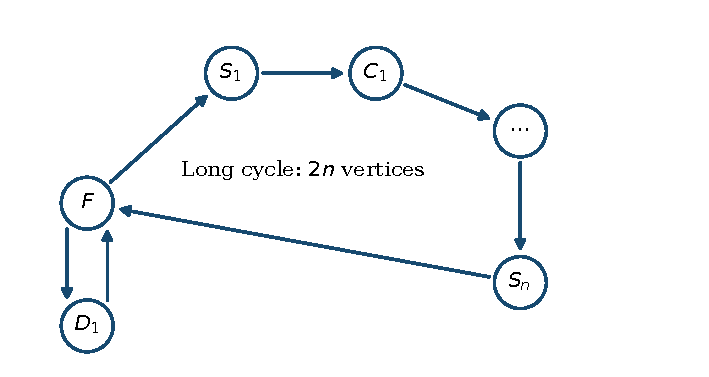
\includegraphics[width=.8\linewidth]{positive_flower.pdf}
\caption{The sign-conjugate matrix $M_n$ as a graph: a long cycle through $2n$ vertices and a two-cycle, sharing the hub $F$. All diagonal entries are $-1$ and all displayed edges have gain $+1$. A positive column scaling multiplies the diagonal loss of a vertex and every edge leaving it by the same rate.}
\label{fig:flower}
\end{figure}

\begin{example}
At $n=2$ the owners are $(F,S_1,C_1,S_2,D_1)$ with reactions $(F_1^b,K_1^b,K_1^v,F_2^b,F_1^v)$: the same five owner--reaction pairs as $S_2$ in \eqref{eq:VScores}, in the order $(S_2,F,D_1,S_1,C_1)$. So $A_2$ is $S_2$ up to simultaneous reordering, and $S_1$ is its image under the kinase--phosphatase symmetry. At $n=3$,
\[
A_3=\begin{pmatrix}
-1&0&0&0&0&-1&-1\\
-1&-1&0&0&0&0&0\\
0&1&-1&0&0&0&0\\
0&0&1&-1&0&0&0\\
0&0&0&1&-1&0&0\\
0&0&0&0&1&-1&0\\
1&0&0&0&0&0&-1
\end{pmatrix},
\]
with $\det(zI-A_3)=z^7+7z^6+20z^5+30z^4+25z^3+11z^2+z-1$.
Each further site inserts one more pair $(S_i,C_i)$ into the long cycle; the family is the iterative extension of $S_2$ in the sense of the conjecture, and its dimension is $2n+1$.
\end{example}

\subsection{Determinant and instability}

\begin{proposition}\label{prop:posdet}
$\det A_n=1$ for every $n\ge2$.
\end{proposition}
\begin{proof}
$\det A_n=\det M_n$. Eliminate the leaf $D_1$ with Lemma~\ref{lem:elimination}: the $1\times1$ block is $-1$ and the Schur complement adds $P_{\text{short}}$'s product $1\cdot1$ to the hub diagonal. The reduced $2n\times2n$ matrix $R$ has hub diagonal $0$, other diagonals $-1$ and the cyclic entries $1$. Expanding $\det R$ along the hub row, whose only nonzero entry is the cyclic $1$ in the last column, and deleting that row and column leaves an upper triangular matrix with unit diagonal (the remaining cycle entries lie on the subdiagonal and the diagonals are $-1$; after deleting the hub row the sub-diagonal entries become the diagonal of the minor). The cofactor sign is $(-1)^{1+2n}=-1$, so $\det R=-1$ and $\det M_n=(-1)^1\det R=1$.
\end{proof}

\begin{proposition}\label{prop:posunstable}
For every $n\ge2$ and every positive diagonal $D$, the matrix $A_nD$ has a positive real eigenvalue. At $D=I$ the positive real eigenvalue $\alpha_n$ is unique, equals $w_n-1$ where $w_n>1$ is the unique real root larger than one of $w^{2n}-w^{2n-2}-1$, and has the eigenvector $u=(w_n^{2n-1},w_n^{2n-2},\dots,w_n,1,\,w_n^{2n-2})^{\T}$ of $M_n$ (cycle coordinates in order, leaf last).
\end{proposition}
\begin{proof}
The order $2n+1$ is odd and $\det(A_nD)=\det D>0$, so $\det(-A_nD)<0$: the monic characteristic polynomial is negative at $0$ and tends to $+\infty$, hence has a positive real root. At unit scaling put $k=2n-1$; the polynomial $f(w)=w^{k+1}-w^{k-1}-1$ satisfies $f(1)=-1<0\le f(2)$, so it has a root $w_n\in(1,2]$, and it is unique on $(1,\infty)$ because $w^{k-1}(w^2-1)$ is strictly increasing there. With $u_i=w_n^{k-i}$ on the cycle ($i=0$ the hub, $i=k$ the last vertex) and $u_\ell=w_n^{k-1}$ on the leaf, the equations of $M_nu=(w_n-1)u$ are $u_{i-1}-u_i=(w_n-1)u_i$ on the chain, $u_0-u_\ell=(w_n-1)u_\ell$ at the leaf, and $u_k+u_\ell-u_0=(w_n-1)u_0$ at the hub; the first two are identities and the third is $1+w_n^{k-1}=w_n^{k+1}$, that is $f(w_n)=0$.
\end{proof}

\subsection{Minimality under every positive scaling}

\begin{lemma}[Contraction along a flower]\label{lem:contraction}
Let $k\ge1$, let $a_0,\dots,a_k,b\in\C$ have real parts greater than one, and let $u_0,\dots,u_k,v\in\C$ satisfy, for a set $P\subseteq\{0,\dots,k\}$ of retained cycle vertices and a flag $\ell\in\{\text{retained},\text{omitted}\}$ for the leaf:
\begin{align*}
&u_i=0\ \text{ for } i\notin P,\qquad v=0\ \text{ if the leaf is omitted},\\
&a_iu_i=u_{i-1}\ \text{ for } i\in P\setminus\{0\},\qquad bv=u_0\ \text{ if the leaf is retained},\qquad a_0u_0=u_k+v\ \text{ if } 0\in P .
\end{align*}
If at least one vertex (cycle vertex or leaf) is omitted, then all $u_i=0$ and $v=0$.
\end{lemma}
\begin{proof}
If $au=u'$ with $\Ree a>1$ then $|u|\le|u'|$ with strict inequality when $u\neq0$, since $|a|\ge\Ree a>1$. Applying this along the chain gives $|u_k|\le|u_{k-1}|\le\dots\le|u_0|$, where an omitted vertex contributes $u_i=0$ and the inequality still holds; the leaf gives $|v|\le|u_0|$. Suppose $u_0\ne0$; then $0\in P$ and $|u_0|<|u_k+v|\le|u_k|+|v|$. If some cycle vertex $i$ is omitted then $|u_k|\le|u_i|=0$, so $|u_0|<|v|\le|u_0|$, impossible. If the leaf is omitted then $v=0$ and $|u_0|<|u_k|\le|u_0|$, impossible. Hence $u_0=0$, and then the chain and leaf inequalities force every $u_i=0$ and $v=0$.
\end{proof}

\begin{proposition}[All-scaling minimality]\label{prop:allrate}
For every $n\ge2$, every positive diagonal $D$ and every proper subset $I'$ of the owners, the restriction $(A_nD)[I']$ is nonunstable.
\end{proposition}
\begin{proof}
By conjugacy it suffices to treat $(M_nD)[I']$. Suppose $(M_nD)[I']v=zv$ with $v\ne0$ and $\Ree z>0$. Extend $v$ by zero to the omitted coordinates and put $u_i=d_iv_i$. For a retained non-hub cycle vertex $i$ the equation reads $u_{i-1}-u_i=zv_i=zu_i/d_i$, that is $(1+z/d_i)u_i=u_{i-1}$, where $u_{i-1}=0$ if $i-1$ is omitted; the retained leaf gives $(1+z/d_\ell)u_\ell=u_h$ and the retained hub gives $(1+z/d_h)u_h=u_{\text{last}}+u_\ell$. Every coefficient $1+z/d_i$ has real part $1+\Ree z/d_i>1$. Since $I'$ is proper, Lemma~\ref{lem:contraction} gives $u=0$, hence $v=0$, a contradiction.
\end{proof}

\begin{proof}[Proof of Theorem~\ref{thm:positive}]
Dimension $2n+1$ and reactant support are immediate from \eqref{eq:posorder}; $\det A_n=1$ is Proposition~\ref{prop:posdet} and $1=(-1)^{2n}$ is the positive sign. For each positive $D$, $A_nD$ is unstable by Proposition~\ref{prop:posunstable} and its proper restrictions are nonunstable by Proposition~\ref{prop:allrate}, so $A_nD$ is an unstable-positive core; $D=I$ gives the core $A_n$, and the same statements give that $A_n$ is a $D$-unstable core. The identification $A_2=S_2$ is the example above.
\end{proof}

\begin{proof}[Proof of Corollary~\ref{cor:resolution}]
(C2) is Theorem~\ref{thm:det}. For (C1), Theorem~\ref{thm:negative} gives a negative core for every $n\ge3$, and Theorem~\ref{thm:positive} at $n=M+1$ gives a minimal unstable-positive core of dimension $2M+3>M$.
\end{proof}

\subsection{Characteristic polynomial and the number of unstable modes}
A permutation of the vertices of $M_n$ decomposes into cycles of its graph; the two nontrivial cycles share the hub and cannot be used together. The cycle-cover expansion of the characteristic polynomial therefore has three terms:
\begin{equation}\label{eq:charpositive}
\det(zI-A_n)=\det(zI-M_n)=(z+1)^{2n+1}-(z+1)^{2n-1}-(z+1),
\end{equation}
the diagonal term, the two-cycle term and the long-cycle term (a $2n$-cycle has sign $-1$, and the leaf contributes its diagonal factor). The script checks \eqref{eq:charpositive} against the exact characteristic polynomial of the literal child for $n\le8$. Positive real roots of \eqref{eq:charpositive} are $w-1$ with $w>1$ and $w^{2n}-w^{2n-2}=1$, unique as shown above, and by Descartes' rule the coefficient sequence has exactly one sign change. A unique positive real eigenvalue does not mean a one-dimensional unstable subspace: for $n=10$ the exact Routh table of the degree-$21$ polynomial has first-column signs $+^{19},-,+,-$, three sign changes and hence three roots in the open right half-plane, one real and one nonreal pair. We do not classify the number of unstable modes for all $n$.

\section{Rates, losses and asymptotics}\label{sec:rates}

The matrices $A_nD$ describe the linearized positive feedback when the selected reactions run at rates $d_i>0$; in a full kinetic model each species is also subject to additional consumption not represented by its owned column. To capture both, let $L$ be the long cycle with hub $h=F$, let $\ell=D_1$ be the leaf, and for rates $d_i>0$ and independent losses $\eta_i\ge0$ put
\begin{equation}\label{eq:H}
H=M_nD-\diag(\eta_i),\qquad a_i=d_i+\eta_i .
\end{equation}
The letter $\eta$ avoids confusion between a loss and the leaf index.

\begin{theorem}[Return equation]\label{thm:return}
There is a unique real $\beta>-\min_ia_i$ with
\begin{equation}\label{eq:return}
\cG(\beta):=\prod_{i\in L}\frac{d_i}{\beta+a_i}+\frac{d_hd_\ell}{(\beta+a_h)(\beta+a_\ell)}=1 ,
\end{equation}
and $\beta$ is the spectral abscissa of $H$: it is an eigenvalue with a strictly positive eigenvector, every other eigenvalue has real part strictly less than $\beta$, and $\beta$ is the only real eigenvalue exceeding $-\min_ia_i$. Sign conjugacy transfers all statements to $TA_nDT-\diag(\eta_i)$. For zero losses write $\alpha_n(d)=\beta$; then $\alpha_n(d)>0$.
\end{theorem}
\begin{proof}
On $(-\min_ia_i,\infty)$ all denominators are positive, both terms of $\cG$ decrease strictly, $\cG\to0$ at $+\infty$, and the term containing a vertex with smallest $a_i$ diverges at the left endpoint; so $\cG=1$ has a unique solution $\beta$ there.

Number the long cycle $h=i_0\to i_1\to\dots\to i_{2n-1}\to h$ and put $u_i=d_iv_i$. The eigenvalue equations $Hv=zv$ are $u_{i_{j-1}}-a_{i_j}v_{i_j}=zv_{i_j}$ along the cycle, $u_h-a_\ell v_\ell=zv_\ell$ at the leaf and $u_{i_{2n-1}}+u_\ell-a_hv_h=zv_h$ at the hub, that is
\begin{equation}\label{eq:propagate}
u_{i_j}=\frac{d_{i_j}}{z+a_{i_j}}u_{i_{j-1}},\qquad u_\ell=\frac{d_\ell}{z+a_\ell}u_h,\qquad u_h=\frac{d_h}{z+a_h}\bigl(u_{i_{2n-1}}+u_\ell\bigr),
\end{equation}
whenever the denominators are nonzero. Starting from $u_h=1$ at $z=\beta$ and propagating, every coordinate is positive and the hub equation becomes exactly $\cG(\beta)=1$; so $\beta$ is an eigenvalue with positive eigenvector. Conversely let $z$ be an eigenvalue with $\Ree z\ge\beta$, so all $z+a_i$ have positive real part. If $u_h=0$ then \eqref{eq:propagate} gives $u=0$; so $u_h\ne0$ and the hub equation yields
\begin{align*}
1&=\prod_{i\in L}\frac{d_i}{z+a_i}+\frac{d_hd_\ell}{(z+a_h)(z+a_\ell)},\qquad\text{hence}\\
1&\le\prod_{i\in L}\frac{d_i}{|z+a_i|}+\frac{d_hd_\ell}{|z+a_h|\,|z+a_\ell|}\le\cG(\Ree z)\le\cG(\beta)=1 ,
\end{align*}
using $|z+a_i|\ge\Ree z+a_i$. Equality forces $\Ree z=\beta$ and $|z+a_i|=\Ree z+a_i$ for the vertices involved, so $\Imm z=0$ and $z=\beta$. The same argument with a real $z>-\min_ia_i$ shows $\cG(z)=1$, so $z=\beta$. Finally $\cG(0)=2$ when all $\eta_i=0$, so $\beta>0$.
\end{proof}

\begin{corollary}[Rate comparisons]\label{cor:rates}
$\alpha_n(d)$ increases strictly with each individual $d_i$, is homogeneous, $\alpha_n(cd)=c\,\alpha_n(d)$ for $c>0$, and satisfies
\begin{equation}\label{eq:ratebounds}
d_{\min}\,\alpha_n(\mathbf 1)\le\alpha_n(d)\le d_{\max}\,\alpha_n(\mathbf 1),\qquad d_{\min}=\min_id_i,\ d_{\max}=\max_id_i .
\end{equation}
\end{corollary}
\begin{proof}
With $\eta=0$ each factor $d_i/(\lambda+d_i)$ increases strictly with $d_i$ at fixed $\lambda>0$, and every vertex occurs in at least one term of \eqref{eq:return}; increasing $d_i$ makes $\cG(\alpha_n(d))>1$ at the old root, so the new root is larger. Replacing $(d,\lambda)$ by $(cd,c\lambda)$ leaves \eqref{eq:return} invariant. Monotonicity in each coordinate then gives \eqref{eq:ratebounds} by comparison with $d_{\min}\mathbf1$ and $d_{\max}\mathbf1$. No entrywise monotonicity of $A_nD$ is used: its negative diagonal changes with the rates too.
\end{proof}

\begin{corollary}[Loss threshold]\label{cor:loss}
Let $G_L=\prod_{i\in L}d_i/(d_i+\eta_i)$ and $G_2=\bigl(d_h/(d_h+\eta_h)\bigr)\bigl(d_\ell/(d_\ell+\eta_\ell)\bigr)$. Then $H$ is strictly stable, has spectral abscissa zero, or is unstable according as $G_L+G_2$ is less than, equal to, or greater than one. A uniform loss $\eta_i=\delta$ for all $i$ gives strict stability if and only if $\delta>\alpha_n(d)$.
\end{corollary}
\begin{proof}
$\cG(0)=G_L+G_2$ and $\cG$ is strictly decreasing, so the sign of $\beta$ is the sign of $\cG(0)-1$. A uniform loss $\delta I$ shifts every eigenvalue by $-\delta$.
\end{proof}

Slowing a column keeps the ratio between the loss of a species and the gain it transmits, while an independent loss changes that ratio; this is why the two interventions enter \eqref{eq:return} differently. These are statements about the selected linear matrix; a full reaction model must realize the intervention before they apply to it.

\subsection{Unit rates: the instability weakens as the cores grow}
At $d=\mathbf1$, $\eta=0$ put $\alpha_n=\alpha_n(\mathbf1)$. Equation \eqref{eq:return} reads
\begin{equation}\label{eq:unitreturn}
(1+\alpha_n)^{-2n}+(1+\alpha_n)^{-2}=1,
\end{equation}
which is $w^{2n}-w^{2n-2}-1=0$ with $w=1+\alpha_n$, as in Proposition~\ref{prop:posunstable}. With $m=n-1$ and $y_n=(1+\alpha_n)^2-1$ it becomes
\begin{equation}\label{eq:y}
y_n(1+y_n)^m=1 .
\end{equation}

\begin{proposition}\label{prop:asymptotic}
The sequence $(\alpha_n)_{n\ge2}$ decreases strictly to zero. Let $r=W(m)>0$ be the Lambert function value defined by $re^r=m$ \citep{Corless1996}. Then $0<r<m$ and
\begin{equation}\label{eq:bracket}
\frac rm\le y_n\le\frac r{m-r},\qquad
\sqrt{1+r/m}-1\le\alpha_n\le\sqrt{1+r/(m-r)}-1 .
\end{equation}
Consequently, as $n\to\infty$,
\begin{equation}\label{eq:asymptotic}
\alpha_n=\frac{W(n-1)}{2(n-1)}+O\!\left(\frac{W(n-1)^2}{(n-1)^2}\right)\sim\frac{\log n}{2n}.
\end{equation}
\end{proposition}
\begin{proof}
For fixed $y>0$ the left side of \eqref{eq:y} increases with $m$ and increases strictly with $y$, so $y_n$ decreases strictly; a positive limit $y_\infty$ would make $y_\infty(1+y_\infty)^m\to\infty$, so $y_n\to0$ and $\alpha_n\to0$.

The function $f_m(y)=\log y+m\log(1+y)$ is strictly increasing and vanishes at $y_n$. From $re^r=m$ with $r>0$ we get $r<m$ and $\log r+r=\log m$. At $u=r/m$, $\log(1+u)\le u$ gives $f_m(u)\le\log(r/m)+r=0$, so $y_n\ge u$. At $v=r/(m-r)$, $\log(1+v)\ge v/(1+v)=r/m$ gives $f_m(v)\ge\log\frac{r}{m-r}+r=\log\frac{m}{m-r}>0$, so $y_n\le v$. This is \eqref{eq:bracket}; the second pair follows from $\alpha_n=\sqrt{1+y_n}-1$.

The bracket has width $r^2/(m(m-r))$, and $r/m\to0$, so $y_n=r/m+O(r^2/m^2)$; expanding $\sqrt{1+y}-1=y/2+O(y^2)$ gives the first formula in \eqref{eq:asymptotic}. Finally $r=\log m-\log r$ and $0<\log r<\log m$ for $m\ge3$ give $\log m-\log\log m\le r\le\log m$, so $W(m)\sim\log m$ and $\alpha_n\sim\log n/(2n)$.
\end{proof}

\begin{table}[htbp]\centering
\caption{The unit-rate unstable eigenvalue $\alpha_n$ of $A_n$, rounded to six decimals, with the Lambert brackets \eqref{eq:bracket}. Time is normalized so that every selected column rate is one. The values illustrate the exact scalar equation and are not proof premises.}\label{tab:alpha}
\begin{tabular}{rrrrr}\toprule
$n$&$\dim A_n$&lower bound&$\alpha_n$&upper bound\\\midrule
2&5&0.251856&0.272020&0.519945\\
3&7&0.194279&0.210608&0.320257\\
5&11&0.140413&0.150964&0.195692\\
10&21&0.089292&0.094300&0.108757\\
25&51&0.047448&0.049036&0.052426\\
100&201&0.016917&0.017139&0.017509\\
\bottomrule
\end{tabular}
\end{table}

\begin{figure}[htbp]\centering
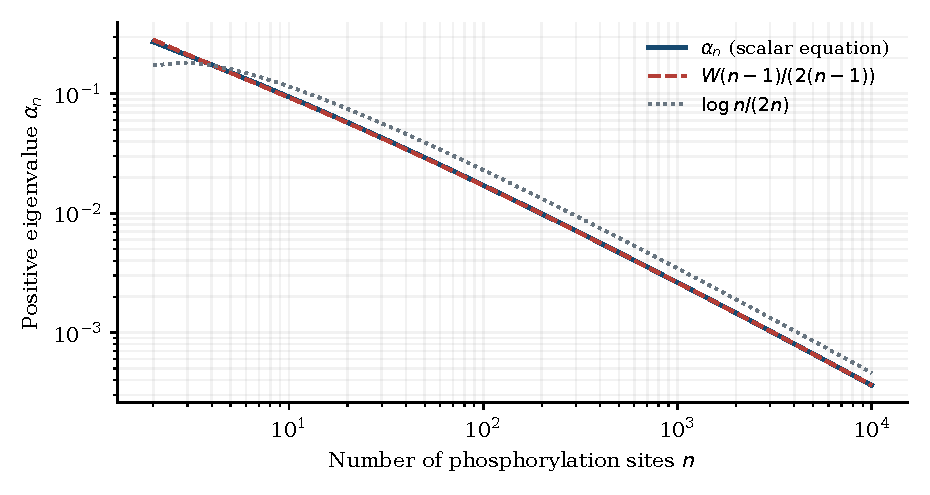
\includegraphics[width=.85\linewidth]{alpha_decay.pdf}
\caption{The unit-rate eigenvalue $\alpha_n$ from \eqref{eq:unitreturn}, the leading Lambert term $W(n-1)/(2(n-1))$ and the logarithmic equivalent, on logarithmic axes. Minimal positive cores of unbounded size coexist with a vanishing dominant instability rate.}\label{fig:alpha}
\end{figure}

\section{A full-network kinetic realization}\label{sec:kinetics}

A child-selection matrix records one derivative per selected species. The theorem of \citep{VassenaStadler2024} converts a $D$-unstable child into an unstable equilibrium for \emph{some} parameter-rich kinetics by an abstract argument. It is instructive to see one explicit realization in which every species and reaction of the network is present. We do this for $n=3$ at the negative core $\Aminus$.

Concentrations and time are nondimensionalized so that the equilibrium is $x^*=\mathbf1$. Assign the fluxes $v_j=4$ to every binding reaction and $v_j=2$ to every unbinding and conversion reaction. In each arm the intermediate balance is $4-2-2=0$, each enzyme is released as fast as it is bound, and each substrate's net production by the kinase arms cancels its net consumption by the phosphatase arms; so $Sv=0$ exactly.

Let $R\in\R^{18\times12}$, rows indexed by reactions and columns by species, have entry $1$ at the six owner--reaction pairs of \eqref{eq:negowners}, entry $\tfrac1{100}$ at every other reactant pair $(j,m)$ with $Y_{mj}>0$, and $0$ elsewhere. Set $\theta_{jm}=R_{jm}/v_j\in(0,1)$ and define the rate laws
\begin{equation}\label{eq:kinetics}
r_j(x)=v_j\prod_{m:\,Y_{mj}>0}\frac{x_m}{\theta_{jm}+(1-\theta_{jm})x_m}.
\end{equation}
Each factor is positive and saturating in $x_m>0$, equals $1$ at $x_m=1$ and has derivative $\theta_{jm}$ there, so $r_j(\mathbf1)=v_j$ and $\partial_mr_j(\mathbf1)=R_{jm}$. The system $\dot x=Sr(x)$ therefore has the positive equilibrium $\mathbf1$ with Jacobian $J=SR$. The construction realizes the prescribed reactivities directly rather than assuming they arise from mass action; it is an effective driven model in which ATP, ADP and phosphate are externally maintained.

\begin{proposition}\label{prop:kinetic}
At the equilibrium $\mathbf1$ the Jacobian $J$ has the eigenvalue $0$ with algebraic multiplicity exactly three, corresponding to the conserved totals
\begin{equation}\label{eq:conservation}
K+\sum_{i=0}^2C_i=4,\qquad F+\sum_{i=1}^3D_i=4,\qquad \sum_{i=0}^3S_i+\sum_{i=0}^2C_i+\sum_{i=1}^3D_i=10,
\end{equation}
and exactly three eigenvalues in the open right half-plane: one positive real root and one nonreal conjugate pair. Every eigenvector with nonzero eigenvalue lies in the complexified stoichiometric subspace $\im_\C S$.
\end{proposition}
\begin{proof}
The three row vectors of \eqref{eq:conservation} annihilate $S$ and $\rank S=9$, so $\rank J\le9$. Exact rational arithmetic gives
\begin{equation}\label{eq:Jpoly}
\det(zI-100J)=z^3q_J(z),
\end{equation}
\begin{align*}
q_J(z)={}&z^9+618z^8+139432z^7+13778512z^6+543179240z^5+14097062574z^4\\
&+1032202684766z^3+3925174058599z^2+3726175329872z-160160507095 .
\end{align*}
The constant term is nonzero, so the multiplicity of the eigenvalue $0$ is exactly three. The exact Routh first column of $q_J$ has signs $+,+,+,+,+,-,+,+,+,-$ and no zero pivot, hence three sign changes and three roots in the open right half-plane; the coefficient sequence has exactly one sign change, so by Descartes' rule there is exactly one positive real root, and the other two unstable roots are a conjugate pair. If $Ju=\lambda u$ with $\lambda\ne0$ then $u=S(Ru/\lambda)\in\im_\C S$.
\end{proof}

Numerically the unstable eigenvalues of $J$ are $0.113319\pm0.389512\,i$ and $0.000411771$; the small positive real eigenvalue is distinct from the three exact zeros. Figure~\ref{fig:spectra} shows the three spectra of this paper side by side. The unstable pair of $J$ is close to the unstable pair $0.142111\pm0.392895\,i$ of $\Aminus$, from which it differs by the $1/100$ background reactivities and the coupling to the other six species; the small additional real unstable eigenvalue has no counterpart in $\Aminus$ and arises from that coupling. We do not attribute it to a particular child selection.

\begin{figure}[htbp]\centering
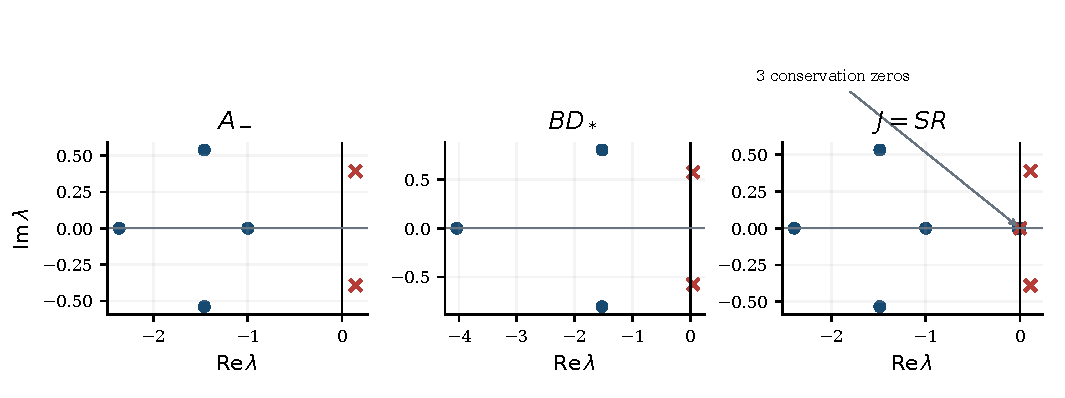
\includegraphics[width=\linewidth]{spectra.pdf}
\caption{Spectra of the unit-scaled negative core $\Aminus$, the scaled five-species core $BD_*$, and the full kinetic Jacobian $J=SR$ of \eqref{eq:kinetics}. Crosses mark eigenvalues with positive real part. The three coincident conservation zeros of $J$ are plotted at one location. All plotted values are numerical illustrations of the exact statements in the text.}\label{fig:spectra}
\end{figure}

The example is neither elementary mass action nor a demonstrated oscillator: it shows that the linear instability located by the child selection is realized at a positive equilibrium of the complete network under an explicit smooth, saturating, flux-balanced kinetics, inside the stoichiometric compatibility class. A Hopf bifurcation would additionally require a parameter-dependent crossing and nonlinear conditions not established here. For the dual cycle under mass action no Hopf bifurcation exists \citep{Vassena2026}; the present example has three sites and non-mass-action rate laws, so there is no conflict, and the mass-action question for $n\ge3$ is open (Section~\ref{sec:discussion}).

\section{Discussion}\label{sec:discussion}

\paragraph{What was resolved.}
The determinant part of the Example D conjecture is a general integrality property of elementary enzyme conversion: after eliminating selected intermediates, only incidence relations among free species remain. The structural part fails, and it fails already at three sites: a fixed six-species negative feedback loop closed through both enzymes appears once there is a third substrate level, and the positive motif $S_2$ of the dual cycle extends to an unstable-positive core of dimension $2n+1$ in the $n$-site cycle. Since every positive scaling of $A_n$ is again a minimal core, the family is robust in the sense relevant to parameter-rich kinetics. On the other hand the instability it carries is weak: at unit rates its unstable eigenvalue is asymptotically $\log n/(2n)$.

\paragraph{Exploratory censuses.}
The script \path{check_paper.py} can enumerate all child selections of the two- and three-site cycles (option \path{--census}) and evaluate their determinants exactly. There are $4455$ children at $n=2$ (determinants $+1$: $535$, $-1$: $543$, $0$: $3377$) and $204849$ at $n=3$ (determinants $+1$: $15641$, $-1$: $15649$, $0$: $173559$), all in $\{0,\pm1\}$ as Theorem~\ref{thm:det} requires. A floating-point screen of the same enumeration (an eigenvalue with real part above $10^{-7}$, and none for any proper restriction) finds at $n=2$ exactly three unstable cores, the matrices $S_1$, $S_2$, $S_3$ of \citep{VassenaStadler2024}, and at $n=3$ finds eighteen unstable cores: six positive cores of dimension five, four positive cores of dimension six, two of dimension seven (the family member $A_3$ and its mirror image) and two of dimension eight, together with four unstable-negative cores of dimension six, among them $\Aminus$. This screen is exploratory: it depends on a tolerance, and only $\Aminus$, $B$ and the family $A_n$ have been certified exactly. It suggests, but does not prove, that $n=3$ is the first cycle with a negative core and that the negative cores of the three-site cycle have dimension at least six.

\paragraph{Relation to the $D$-core conjecture.}
Vassena and Stadler also conjectured that a network without $D$-unstable cores admits no instability under parameter-rich kinetics. That conjecture is refuted in the companion manuscripts \citep{ParameterRich2026,KineticOrder2026}, which construct networks whose instability is not localized by any child selection. The present paper is complementary: in the futile cycle the child-selection framework does localize instability, and the question is which cores occur. The five-species core $B$ shows that the $D$-unstable cores of a network can be strictly smaller than its unstable cores, and that a strictly stable child can become the certificate of instability after rescaling two of its columns.

\paragraph{Open questions.}
\begin{enumerate}[label=(\roman*)]
\item \emph{Classification up to subdivision.} Read modulo subdivision of the long cycle, the family $A_n$ is one template. Are all unstable-positive cores of the $n$-site cycle subdivisions of $S_1=S_2$ or $S_3$, and are all unstable-negative cores subdivisions of $\Aminus$? The censuses above are the natural first test; a proof would need a structural description of all children with a unique unstable cycle.
\item \emph{Unstable dimension.} $A_n$ has one unstable eigenvalue for $n=2,3$ and three for $n=10$. The exact number for every $n$, and its growth, is not determined here; \eqref{eq:charpositive} reduces it to a Routh--Hurwitz question for the polynomial $w^{2n+1}-w^{2n-1}-w$.
\item \emph{Mass action.} Does the $n$-site cycle with $n\ge3$ admit a Hopf bifurcation or an unstable positive equilibrium under mass-action kinetics? The negative core $\Aminus$ is a candidate mechanism, but a child selection determines neither the mass-action Jacobian nor its conservation constraints \citep{KineticOrder2026}, and the dual-cycle exclusion \citep{Vassena2026} shows that structural capacity under parameter-rich kinetics can disappear under mass action.
\item \emph{Smallest negative cores.} Is six the minimal dimension of an unstable-negative core in any $n$-site cycle, and is five the minimal dimension of a $D$-unstable-negative core?
\end{enumerate}

\appendix

\section{Formal verification}\label{app:formal}

The Lean~4 development is a set of modules in the namespace \lean{FutileCycle}, built against a frozen Mathlib with toolchain \lean{leanprover/lean4:v4.30.0}. The source network is defined literally: \lean{ConversionSystem} carries the maps $s,t,e$ on an arbitrary intermediate type, \lean{futile n} instantiates it for \eqref{eq:network}, and \lean{Child} packages an injective species map, an injective reaction map and the reactant-support condition; \lean{Child.matrix} is \eqref{eq:child}. The predicates \lean{MinimalUnstable} (unstable, every proper principal restriction nonunstable), \lean{DUnstable} and \lean{DNonUnstable} are those of Definition~\ref{def:core}, with instability stated as the existence of a complex eigenpair with positive real part. No numerical eigenvalue, floating computation or generated case file is a premise of any theorem; the finite mask theorem for the negative core is evaluated by the kernel.

\begin{table}[htbp]\centering\small
\caption{Statements of this paper and their formal counterparts. Files are under \texttt{proofs/FutileCycle/}.}\label{tab:formal}
\begin{tabular}{>{\raggedright\arraybackslash}p{.34\linewidth}>{\raggedright\arraybackslash}p{.60\linewidth}}\toprule
Statement & Declaration (file)\\\midrule
Lemma~\ref{lem:incidence} & \lean{incidence_det_bound} (\path{IncidenceDeterminant.lean})\\
Lemma~\ref{lem:elimination} & \lean{det_intermediate_elimination} (\path{IntermediateElimination.lean})\\
Reduced columns \eqref{eq:reduced} & \lean{reducedColumns_signedIncidence} (\path{ReducedColumns.lean})\\
Theorem~\ref{thm:det}, general class & \lean{child_det_bound} (\path{AllNDeterminant.lean})\\
Theorem~\ref{thm:det}, futile cycle & \lean{allN_child_det} (\path{AllNDeterminant.lean})\\
Lemma~\ref{lem:reciprocal} & \lean{exists_rhp_root_of_reciprocal_sum} (\path{ReciprocalInstability.lean})\\
Proposition~\ref{prop:neginstability} & \lean{negativeQuintic_rhp}, \lean{negative_unstable} (\path{NegativeSpectrum.lean})\\
Lemma~\ref{lem:lyapunov} & \lean{lyapunovQ_gram}, \lean{exceptional_lyapunov_identity}, \lean{exceptional_no_rhp} (\path{ExceptionalRestriction.lean}, \path{Lyapunov.lean})\\
Minimality of $\Aminus$ & \lean{negative_principal_no_rhp} (\path{NegativeMinimality.lean}), with \lean{negativeMasked_annihilator}, \lean{annihilator_no_rhp}, \lean{mask_coverage}, \lean{principal_eigenpair_extends}\\
Theorem~\ref{thm:negative} & \lean{negative_core_all_n} (\path{NegativeCore.lean}), embedding \lean{negativeChildAt_matrix} (\path{NegativeEmbedding.lean})\\
Lemma~\ref{lem:logderivative} & \lean{rhp_of_log_derivative} (\path{NegativeFive.lean})\\
Theorem~\ref{thm:five}, existence and restrictions & \lean{negativeFive_scaled_unstable}, \lean{negativeFive_core_all_n} (\path{NegativeFive.lean}, \path{NegativeFiveMinimality.lean})\\
Source child \eqref{eq:posorder} & \lean{positiveChild}, \lean{positive_dimension} (\path{PositiveSource.lean})\\
Sign conjugacy \eqref{eq:flower} & \lean{positive_source_flower} (\path{PositiveStructure.lean}), \lean{sign_conjugate_det}, \lean{sign_conjugate_eigenpair} (\path{SignConjugacy.lean})\\
Proposition~\ref{prop:posdet} & \lean{flowerMatrix_det}, \lean{positive_det} (\path{FlowerMatrix.lean}, \path{PositiveCore.lean})\\
Proposition~\ref{prop:posunstable} & \lean{flower_eigenpair} (\path{FlowerSpectrum.lean}), \lean{positive_unstable}, \lean{positive_all_rates} (\path{PositiveAllRates.lean})\\
Lemma~\ref{lem:contraction} & \lean{flower_restriction_zero} (\path{FlowerMinimality.lean})\\
Proposition~\ref{prop:allrate} & \lean{flower_scaled_no_rhp}, \lean{positive_proper_scaling} (\path{FlowerScaledMinimality.lean}, \path{PositiveCore.lean})\\
Theorem~\ref{thm:positive} & \lean{positive_core_all_n}, \lean{positive_all_rates_minimal} (\path{Resolution.lean}, \path{PositiveAllRates.lean})\\
Corollary~\ref{cor:resolution} & \lean{resolution}, \lean{not_all_positive}, \lean{no_literal_positive_bound} (\path{Resolution.lean})\\
\bottomrule
\end{tabular}
\end{table}

The aggregate theorem \lean{FutileCycle.resolution} states the conjunction of the determinant claim for all $n$, the existence of a six-species minimal unstable child with determinant $1$ for all $n\ge3$, the existence of a minimal unstable child of dimension $2n+1$ with determinant $1$ for all $n\ge2$, the negation of the all-positive claim, and the negation of every literal dimension bound. Its verification receipt, and those of \lean{positive_all_rates_minimal} and \lean{negativeFive_core_all_n}, record exit code $0$, warnings treated as errors, no \lean{sorry}, and the axiom sets $\{$\lean{Classical.choice}, \lean{Quot.sound}, \lean{propext}$\}$ for every exported declaration. Source SHA-256 prefixes of the three endpoint files at verification were \lean{273d8713} (\path{Resolution.lean}), \lean{76196f57} (\path{PositiveAllRates.lean}) and \lean{7dcbe248} (\path{NegativeFiveMinimality.lean}).

\paragraph{Conventional statements.}
The following are proved in the text and replayed exactly by \path{check_paper.py} but are not Lean declarations: the exact Routh root counts for $\Aminus$, $BD_*$, the $n=10$ member of the positive family and the kinetic Jacobian; the cycle enumeration of Section~\ref{sec:negative} as stated (Lean proves the same spectral conclusion by the annihilator theorem); the characteristic polynomial identity \eqref{eq:charpositive} (Lean uses the explicit eigenvector instead); Theorem~\ref{thm:return} with Corollaries~\ref{cor:rates}--\ref{cor:loss}; Proposition~\ref{prop:asymptotic}; and Proposition~\ref{prop:kinetic} with the rate-law construction \eqref{eq:kinetics}.

\section{Exact certificates}\label{app:cert}

For a descending coefficient list $a_0,\dots,a_m$ the Routh table places the even- and odd-indexed coefficients in its first two rows and continues with $R_{i,j}=(R_{i-1,0}R_{i-2,j+1}-R_{i-2,0}R_{i-1,j+1})/R_{i-1,0}$; when no first-column entry vanishes, the number of sign changes in the first column equals the number of roots in the open right half-plane \citep[Chapter~XV]{Gantmacher1959}. All tables below were computed in exact rational arithmetic and have no zero pivot.
\begin{align*}
\det(zI-\Aminus)&:\ 1,\ 6,\ 11,\ \tfrac{109}{11},\ \tfrac{2177}{654},\ -\tfrac{5491}{2177},\ 1 && \text{two sign changes;}\\
\det(zI-B)&:\ 1,\ 5,\ \tfrac{38}{5},\ \tfrac{221}{38},\ \tfrac{109}{221},\ 1 && \text{no sign change;}\\
\det(zI-BD_*)&:\ 1,\ 7,\ \tfrac{92}{7},\ \tfrac{257}{23},\ -\tfrac{328}{257},\ 4 && \text{two sign changes;}\\
q_J&:\ +,+,+,+,+,-,+,+,+,- && \text{three sign changes;}\\
\det(zI-A_{10})&:\ +^{19},-,+,- && \text{three sign changes.}
\end{align*}
The complete rational first columns of the last two, the matrices $S$, $R$, $J$ and $Q$, the $LDL^{\T}$ pivots of $Q$, the eigenvector residuals, the reconstruction of $S_1,S_2,S_3$ from \eqref{eq:network}, the identity $T A_nT=M_n$ and \eqref{eq:charpositive} for $n\le8$, the Lambert brackets of Table~\ref{tab:alpha} and the flux, conservation and rank statements of Section~\ref{sec:kinetics} are all checked by \path{check_paper.py}; the exact values are also stored in \path{exact_certificates.json}. The vector figures are produced by \path{make_figures.py} from the same data.

\bibliographystyle{plainnat}
\bibliography{refs}

\end{document}
